\documentclass[letterpaper,11pt]{report}

\usepackage[utf8]{inputenc}

%idioma
\usepackage[spanish]{babel}
\selectlanguage{spanish}

%Apendice
\usepackage[toc,page]{appendix}

%formato de bibliografia y citas
\usepackage{cite}
%\usepackage{apacite}
 
\usepackage[nottoc]{tocbibind}

\usepackage{etoc}
\usepackage{blindtext}

%Imagenes
\usepackage{graphicx}
\graphicspath{{./images/}}
%\usepackage[font=small,skip=20pt]{caption}
\setlength{\abovecaptionskip}{15pt plus 5pt minus 2pt}

%Espacio de interlineado
\usepackage{setspace}
\thispagestyle{empty}
\doublespacing
%\onehalfspacing

%Tamaño de márgenes
\usepackage[left=1.25in, right=1.25in]{geometry}
\usepackage{layout}
\usepackage{showframe}
\setlength{\marginparwidth}{0pt}
\setlength{\marginparsep}{0pt}
%\setlength{\textheight}{610pt}

%Colores en el texto
\usepackage{xcolor}

% Incluir subsubsection en el índice
\setcounter{secnumdepth}{3}
\setcounter{tocdepth}{3}

% Landscape pages on demand
\usepackage{lscape}


% tablas
\usepackage{longtable} % Long tables
\usepackage{rotating} % To display tables in landscape
\usepackage{multirow} % Multirows
\usepackage{tabto}

\begin{document}
\layout 
\tableofcontents

\chapter{Diseño del proyecto}\label{cap3}
Conforme a lo visto en el capítulo anterior, el proyecto requiere ser ejecutado de dos formas distintas (ejecución de automatizaciones y portal de usuario), además necesita de una base de datos para mantener persistentes los datos de las órdenes de reposición atendidas, catálogos y datos de usuario, también es necesario acceso al sistema de archivo para guardar las capturas de pantalla de las órdenes de reposición enviadas. Por lo que es necesario dos ambientes de ejecución, la automatización que será ejecutada exclusivamente en el sistema operativo y la del web, que si bien también estará contenida en el sistema operativo es necesario que se ejecute parte del sistema en el explorador del usuario.


%===============================================================================
%===============================================================================


\section{Diseño de la arquitectura}
Bourque define la arquitectura de software como:\footnote{\textcolor{red}{Karla, como es cita textual (según mi propia traducción :P ) prefiero dejarla en un párrafo por separado mientras que lo que sea paráfrasis dejarlo en texto seguido ¿cómo ves?}}
\begin{quote}
	El conjunto de estructuras necesarias para la comprensión de un sistema en el cual se comprometen elementos de software, relaciones entre ellos y sus propiedades\cite{SWEBOOK}.
\end{quote}
En las últimas décadas la arquitectura de software ha profundizado en el estudio genérico de las estructuras del software, dando lugar a técnicas como Patrones de Diseño, Arquitectura 4+1, Arquitectura Orientada a Servicios\cite{SWEBOOK, SoftwareArchitectureInAction}.
\paragraph{Arquitectura Orientada a Servicios:}
Thomas Erl describe la Arquitectura Orientada a Servicios (\textbf{SOA} por sus siglas en inglés) como el modelo arquitectónico del cómputo orientado a servicios\cite{SOAWithRest}, a continuación se muestran las definiciones de Erl sobre los conceptos de Orientación a Servicios:
\begin{quote}
La \textbf{Orientación a Servicios} es el paradigma de diseño dedicado para la creación de unidades lógicas de solución que son moldeados individualmente para que puedan ser utilizados colectiva y repetidamente para la realización de objetivos estratégicos y beneficios asociados con el cómputo orientado a servicios.\\
El \textbf{Cómputo Orientado a Servicios} es engloba distintas plataformas de cómputo distribuido. En sí envuelve su propio paradigma y principios de diseño, catálogos de diseño de patrones, lenguajes, modelo arquitectónico junto con sus conceptos relacionados, tecnologías y marcos de trabajo.\\
La \textbf{Arquitectura Orientada a Servicios} es un modelo de tecnología arquitectónica para soluciones orientadas a servicios con distintas características en apoyo de realizar orientación a servicios y los objetivos estratégicos asociados con el cómputo orientado a servicios.\cite{SOAWithRest}
\end{quote}

\textcolor{red}{Mencionar los patrones de diseño SOA utilizados, apéndice de SOA with REST }\\
\textcolor{red}{Escribir por qué SOA nos favorece.}

\paragraph{Patrones de Diseño:}
\begin{quote}
Un patrón describe un problema recurrente sobre un ambiente, y entonces describe la técnica que soluciona el problema de forma tal que puede ser utilizado sobre cualquier instancia del problema\cite{DesignPatterns}
\end{quote}
Es decir, dados los requerimientos funcionales del sistema es posible analizar la comunicación entre sus distintas partes y de esta forma saber lo patrones que son útiles para dar solución. De acuerdo con Gamma los patrones son organizados en tres categorías\cite{DesignPatterns}:
\begin{enumerate}
	\item \textbf{Creacionales}: describen la forma en que las entidades (objetos si se utiliza el paradigma orientado a objetos) del sistema son creadas.
	\item \textbf{Estructurales}: describen la organización entre las entidades del sistema.
	\item \textbf{Comportamiento}: describen la comunicación entre entidades del sistema
\end{enumerate}


\subsection{Componentes del sistema AutoSA}
El diagrama de componentes sirve para visualizar los componentes en los que se divide el sistema y las interfaces por las cuales se comunican tales componentes, el la Figura \ref{fig:dia-components} se muestra el diagrama de componentes para el sistema AutoSA. En las secciones consecuentes se describe cada componente y las interfaces que ofrece\footnote{Únicamente se mostrarán los diagramas de secuencia más completos que reflejan un comportamiento no trivial.}.
\begin{figure}[h]
\centering
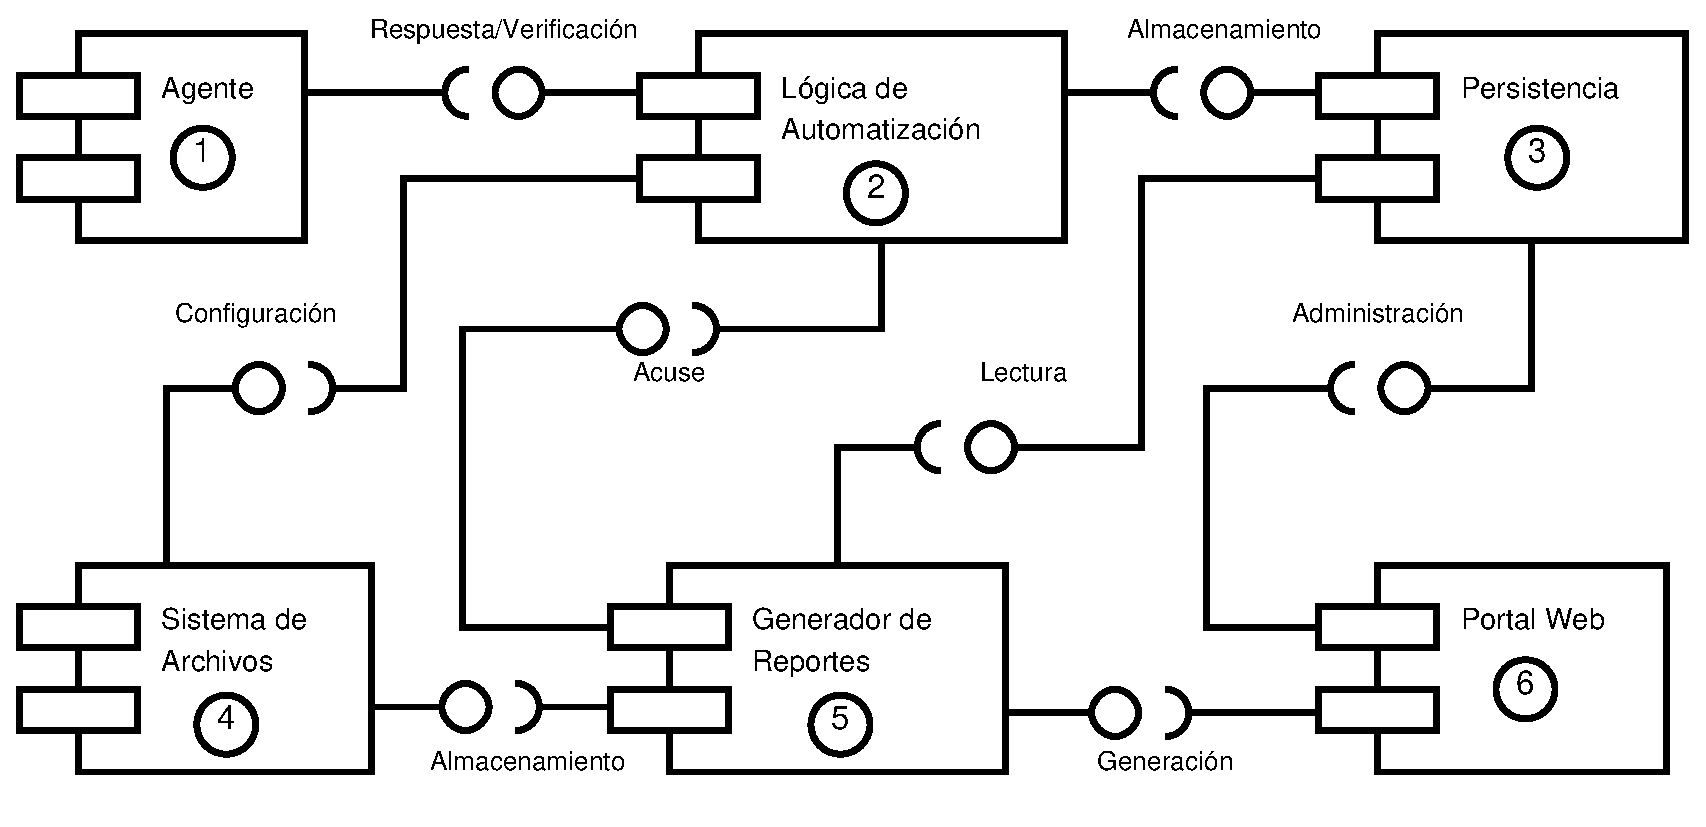
\includegraphics[width=\textwidth]{dia-components}
\caption{Diagrama de componentes.}
\label{fig:dia-components}
\end{figure}

\subsubsection{Agente}
El componente que contiene y ejecuta las rutinas de automatización, esto es mediante una interfaz con el usuario en la cual puede seleccionar el proceso a ser ejecutado. No ofrece interfaces a los demás componentes, consume exclusivamente el componente de Lógica de Automatización.\\

\subsubsection{Lógica de Automatización}
La función de este componente es de ejecutar las reglas de negocio necesarias para en los flujos de los procesos de automatización.  
\paragraph{Respuesta:}
Provee el acceso a las reglas de negocio del proceso de respuesta de órdenes de reposición (ver caso de uso \ref{cu-contestar}).
	\vspace{5mm}\\
	\begin{tabular}{|p{\dimexpr.16\textwidth}|p{\dimexpr.84\textwidth-4\tabcolsep}|}
		\hline
		\textbf{Identificador}	& \textbf{guardar-orden-nueva}\\
		\hline
		\hline
		\textbf{Descripción}	& Guarda un listado de nuevas órdenes de reposición.\\
		\hline
		\textbf{Parámetros}		& \textbullet\, Listado de mapas, cada mapa contiene los datos de una orden de reposición.\\
		\hline
		\textbf{Resultado}		& No ofrece resultado.\\
		\hline
	\end{tabular}
	\vspace{5mm}\\
	\begin{tabular}{|p{\dimexpr.16\textwidth}|p{\dimexpr.84\textwidth-4\tabcolsep}|}
		\hline
		\textbf{Identificador}	& \textbf{obtener-orden-contestar}\\
		\hline
		\hline
		\textbf{Descripción}	& Da la siguiente orden de reposición para contestar.\\
		\hline
		\textbf{Parámetros}		& \textbullet\, No recibe parámetros.\\
		\hline
		\textbf{Resultado}		& Mapa con la información de la orden de reposición.\\
		\hline
	\end{tabular}
	\vspace{5mm}\\
	\begin{tabular}{|p{\dimexpr.16\textwidth}|p{\dimexpr.84\textwidth-4\tabcolsep}|}
		\hline
		\textbf{Identificador}	& \textbf{obtener-datos-respuesta}\\
		\hline
		\hline
		\textbf{Descripción}	& Da los datos necesarios para llenar los formularios para contestar una orden de reposición en el Sistema de Abastecimiento.\\
		\hline
		\textbf{Parámetros}		& \textbullet\, Mapa con los datos de la orden para contestar.\\
		\hline
		\textbf{Resultado}		& Mapa con la información para llenar los formularios para contestar la orden de reposición.\\
		\hline
	\end{tabular}
	\vspace{5mm}\\
	\begin{tabular}{|p{\dimexpr.16\textwidth}|p{\dimexpr.84\textwidth-4\tabcolsep}|}
		\hline
		\textbf{Identificador}	& \textbf{actualizar-orden-contestada}\\
		\hline
		\hline
		\textbf{Descripción}	& Actualiza los datos guardados de la orden de reposición con los datos de la respuesta en el  Sistema de Abastecimiento. Utiliza el componente de persistencia para actualizar los datos.\\
		\hline
		\multirow{2}{*}{\textbf{Parámetros}}	& \textbullet\, Número de orden.\\
												& \textbullet\, Mapa con los datos para guardar.\\
		\hline
		\textbf{Resultado}		& No ofrece resultado.\\
		\hline
	\end{tabular}
	\vspace{5mm}\\
	\begin{tabular}{|p{\dimexpr.16\textwidth}|p{\dimexpr.84\textwidth-4\tabcolsep}|}
		\hline
		\textbf{Identificador}	& \textbf{obtener-orden-enviar}\\
		\hline
		\hline
		\textbf{Descripción}	& Da la siguiente orden de reposición para enviar.\\
		\hline
		\textbf{Parámetros}		& \textbullet\, No recibe parámetros.\\
		\hline
		\textbf{Resultado}		& Mapa con la información de la orden de reposición.\\
		\hline
	\end{tabular}
	\vspace{5mm}\\
	\begin{tabular}{|p{\dimexpr.16\textwidth}|p{\dimexpr.84\textwidth-4\tabcolsep}|}
		\hline
		\textbf{Identificador}	& \textbf{guardar-orden-enviada}\\
		\hline
		\hline
		\textbf{Descripción}	& Actualiza los datos guardados de la orden de reposición con los datos de la pantalla de envío del Sistema de Abastecimiento. Utiliza el componente de persistencia para actualizar los datos.\\
		\hline
		\multirow{2}{*}{\textbf{Parámetros}}	& \textbullet\, Número de orden.\\
												& \textbullet\, Mapa con los datos para guardar.\\
		\hline
		\textbf{Resultado}		& No ofrece resultado.\\
		\hline
	\end{tabular}
	\vspace{5mm}\\
	\begin{tabular}{|p{\dimexpr.16\textwidth}|p{\dimexpr.84\textwidth-4\tabcolsep}|}
		\hline
		\textbf{Identificador}	& \textbf{obtener-acuse-envio}\\
		\hline
		\hline
		\textbf{Descripción}	& Solicita la generación de el acuse de envío al componente de reportes y almacena el documento el componente de Sistema de Archivos.\\
		\hline
		\textbf{Parámetros}		& \textbullet\, Número de orden.\\
		\hline
		\textbf{Resultado}		& No ofrece resultado.\\
		\hline
	\end{tabular}
	\vspace{5mm}
\paragraph{Verificación\\}
Provee el acceso a las reglas de negocio del proceso de verificación de órdenes de reposición canceladas.
	\vspace{5mm}\\
	\begin{tabular}{|p{\dimexpr.16\textwidth}|p{\dimexpr.84\textwidth-4\tabcolsep}|}
		\hline
		\textbf{Identificador}	& \textbf{obtener-rango-fechas-verificar}\\
		\hline
		\hline
		\textbf{Descripción}	& Obtiene el rango de fechas para ingresar en el formulario de búsqueda del Sistema de Abastecimiento. El número de días que comprende el rango se obtiene utilizando el componente de Sistema de archivos.\\
		\hline
		\textbf{Parámetros}		& \textbullet\, No tiene parámetros.\\
		\hline
		\textbf{Resultado}		& El número de días para el rango de búsqueda.\\
		\hline
	\end{tabular}
	\vspace{5mm}\\
	\begin{tabular}{|p{\dimexpr.16\textwidth}|p{\dimexpr.84\textwidth-4\tabcolsep}|}
		\hline
		\textbf{Identificador}	& \textbf{actualizar-estado-sa}\\
		\hline
		\hline
		\textbf{Descripción}	& Actualiza el EstadoSA de las órdenes de reposición recibidas a \textbf{Cancelada}. Utiliza el componente de persistencia para la actualización de datos.\\
		\hline
		\textbf{Parámetros}		& \textbullet\, Listado con los números de las órdenes de reposición canceladas.\\
		\hline
		\textbf{Resultado}		& El número de órdenes de reposición actualizadas.\\
		\hline
	\end{tabular}
	\vspace{5mm}

\subsubsection{Persistencia}
El componente de persistencia está basado en el patrón de diseño \textit{DAO}\footnote{Ver apéndice \ref{sec-dao}}\footnote{En adelante se utilizará \textbf{DAO} para hacer referencia al patrón y la instancia (objeto) del patrón.} para controlar el acceso a la base de datos.\\
El componente de persistencia de el proyecto AutoSA presenta las siguientes interfaces de búsqueda y almacenamiento:
\paragraph{Almacenamiento\\}
Conjunto de operaciones diseñadas para responder a las necesidades de almacenamiento en los flujos para responder y verificar órdenes de reposición\footnote{Ver casos de uso \ref{cu-contestar}, \ref{cu-guardar-nueva}, \ref{cu-responder-orden}, \ref{cu-enviar-orden} y \ref{cu-actualizar-estatus-sa}.}:
	\vspace{5mm}\\
	\begin{tabular}{|p{\dimexpr.16\textwidth}|p{\dimexpr.84\textwidth-4\tabcolsep}|}
		\hline
		\textbf{Identificador}	& \textbf{guardar-nueva} \\
		\hline
		\hline
		\textbf{Descripción}	& Inserta una nueva orden de reposición en la base de datos como se muestra en la figura \ref{fig:dia-seq-store-save-new}.\\
		\hline
		\textbf{Parámetros} 	& \textbullet\, Mapa con los datos de la orden de reposición.\\
		\hline
		\textbf{Resultado}		& No ofrece resultado.\\
		\hline
	\end{tabular}
	\vspace{5mm}\\
	\iffalse
	\begin{figure}[h]
		\centering
		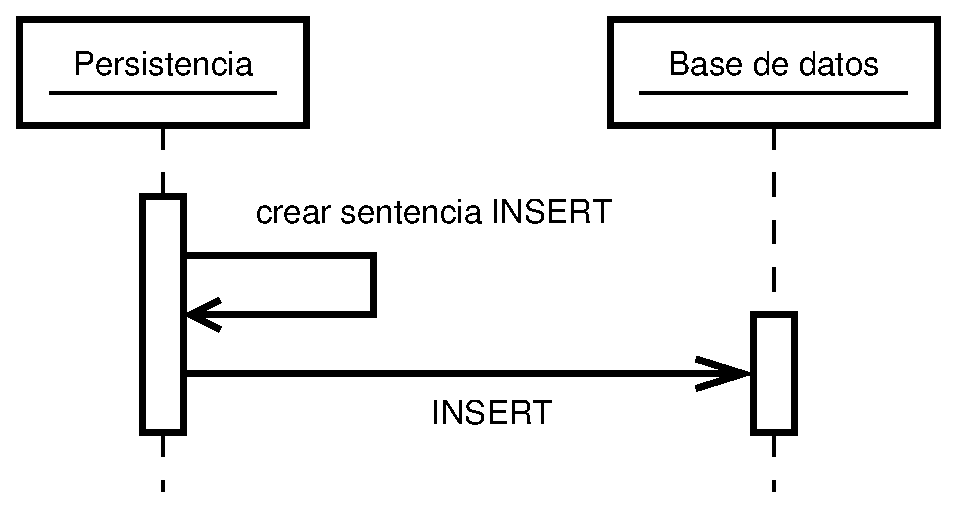
\includegraphics[scale=0.4]{dia-seq-store-save-new}
		\caption{Diagrama de secuencia de la operación guardar-nueva de la interfaz Almacenamiento.}
		\label{fig:dia-seq-store-save-new}
	\end{figure}
	\fi
%	\vspace{5mm}\\
	\begin{tabular}{|p{\dimexpr.16\textwidth}|p{\dimexpr.84\textwidth-4\tabcolsep}|}
		\hline
		\textbf{Identificador}	& \textbf{cambiar-estado} \\
		\hline
		\hline
		\textbf{Descripción}	& Cambia el estado de atención de una orden de reposición. \\
		\hline
		\multirow{2}{*}{\textbf{Parámetros}}	& \textbullet\, Número de orden de reposición.\\
												& \textbullet\, Estado.\\
		\hline
		\textbf{Resultado}		& No ofrece resultado.\\
		\hline
	\end{tabular}
	\vspace{5mm}\\
	\begin{tabular}{|p{\dimexpr.16\textwidth}|p{\dimexpr.84\textwidth-4\tabcolsep}|}
		\hline
		\textbf{Identificador}	& \textbf{guardar-respuesta}\\
		\hline
		\hline
		\textbf{Descripción}	& Guarda los datos de los formularios de la pantalla de respuesta de las órdenes de reposición.\\
		\hline
		\multirow{2}{*}{\textbf{Parámetros}}	& \textbullet\, Número de orden de reposición.\\
												& \textbullet\, Mapa con los datos de los formularios.\\
		\hline
		\textbf{Resultado}		& No ofrece resultado.\\
		\hline
	\end{tabular}
	\vspace{5mm}\\
	\begin{tabular}{|p{\dimexpr.16\textwidth}|p{\dimexpr.84\textwidth-4\tabcolsep}|}
		\hline
		\textbf{Identificador}	& \textbf{guardar-folio-acuse}\\
		\hline
		\hline
		\textbf{Descripción}	& Guarda el folio de acuse de envío de la orden de reposición.\\
		\hline
		\multirow{2}{*}{\textbf{Parámetros}} 	& \textbullet\, Número de orden de reposición.\\
												& \textbullet\, Folio de acuse de envío.\\
		\hline
		\textbf{Resultado}		& No ofrece resultado.\\
		\hline
	\end{tabular}
	\vspace{5mm}\\
	\begin{tabular}{|p{\dimexpr.16\textwidth}|p{\dimexpr.84\textwidth-4\tabcolsep}|}
		\hline
		\textbf{Identificador}	& \textbf{actualizar-estado-sa}\\
		\hline
		\hline
		\textbf{Descripción}	& Actualiza el estado de atención en el Sistema de Abastecimiento a \textbf{cancelada} de las órdenes de reposición recibidas.\\
		\hline
		\textbf{Parámetros} 	& \textbullet\, Lista con los números de las órdenes de reposición.\\
		\hline
		\textbf{Resultado}		& El número de órdenes de reposición actualizadas.\\
		\hline
	\end{tabular}
	\vspace{5mm}\\
	\begin{tabular}{|p{\dimexpr.16\textwidth}|p{\dimexpr.84\textwidth-4\tabcolsep}|}
		\hline
		\textbf{Identificador}	& \textbf{registrar-evento}\\
		\hline
		\hline
		\textbf{Descripción}	& Registra en la base de datos un evento que ocurre durante los procesos automatizados, el evento puede ser de carácter informativo o de error.\\
		\hline
		\multirow{2}{*}{\textbf{Parámetros}}	& \textbullet\, Tipo de evento.\\
												& \textbullet\, Mapa con la descripción del evento.\\
		\hline
		\textbf{Resultado}		& No ofrece resultado.\\
		\hline
	\end{tabular}
	\vspace{5mm}

\paragraph{Lectura\\}
Conjunto de operaciones diseñadas para las necesidades de lectura de órdenes de reposición en los flujos para responder y verificar órdenes de reposición\footnote{Ver casos de uso \ref{cu-contestar}, \ref{cu-enviar-orden} y \ref{cu-generar-acuse}.}:
	\vspace{5mm}\\
	\begin{tabular}{|p{\dimexpr.16\textwidth}|p{\dimexpr.84\textwidth-4\tabcolsep}|}
		\hline
		\textbf{Identificador}	& \textbf{siguiente-orden-contestar}\\
		\hline
		\hline
		\textbf{Descripción}	& Entrega un mapa con los datos de la primera orden de reposición encontrada con estado \textbf{Nueva}.\\
		\hline
		\textbf{Parámetros} 	& \textbullet\, No tiene parámetros.\\
		\hline
		\textbf{Resultado}		& Un mapa con los datos de la primera orden de reposición encontrada con estado \textbf{Nueva}. En caso de no existir tal orden regresa un mapa vacío.\\
		\hline
	\end{tabular}
	\vspace{5mm}\\
	\begin{tabular}{|p{\dimexpr.16\textwidth}|p{\dimexpr.84\textwidth-4\tabcolsep}|}
		\hline
		\textbf{Identificador}	& \textbf{obtener-datos-acuse}\\
		\hline
		\hline
		\textbf{Descripción}	& Obtiene los datos de una orden de reposición necesarios para generar el documento de acuse de envío.\\
		\hline
		\textbf{Parámetros}		& \textbullet\, Número de orden de reposición.\\
		\hline
		\textbf{Resultado}		& Un mapa con los datos de la orden de reposición. En caso de no existir tal orden regresa un mapa vacío.\\
		\hline
	\end{tabular}
	\vspace{5mm}\\
	\begin{tabular}{|p{\dimexpr.16\textwidth}|p{\dimexpr.84\textwidth-4\tabcolsep}|}
		\hline
		\textbf{Identificador}	& \textbf{siguiente-orden-enviar}\\
		\hline
		\hline
		\textbf{Descripción}	& Entrega un mapa con los datos de la primera orden de reposición encontrada con estado \textbf{Contestada}.\\
		\hline
		\textbf{Parámetros} 	& \textbullet\, No tiene parámetros.\\
		\hline
		\textbf{Resultado}		& Un mapa con los datos de la primera orden de reposición encontrada con estado \textbf{Contestada}. En caso de no existir tal orden regresa un mapa vacío.\\
		\hline
	\end{tabular}
	\vspace{5mm}

\paragraph{Administración\\}
Son las operaciones que permiten modificar datos específicos de las órdenes de reposición contenidas en la base de datos, también ofrece la actualización masiva de catálogos\footnote{Ver casos de uso \ref{cu-entrar-web}, \ref{cu-generar-reporte}, \ref{cu-actualizar-catalogo}, \ref{cu-buscar}, \ref{cu-visualizar} y \ref{cu-editar}.}).
	\vspace{5mm}\\
	\begin{tabular}{|p{\dimexpr.16\textwidth}|p{\dimexpr.84\textwidth-4\tabcolsep}|}
		\hline
		\textbf{Identificador}	& \textbf{buscar-credenciales}\\
		\hline
		\hline
		\textbf{Descripción}	& Busca las credenciales del usuario.\\
		\hline
		\textbf{Parámetros}		& \textbullet\, Identificador de usuario.\\
		\hline
		\textbf{Resultado}		& Un mapa con las credenciales del usuario.\\
		\hline
	\end{tabular}
	\vspace{5mm}\\
	\begin{tabular}{|p{\dimexpr.16\textwidth}|p{\dimexpr.84\textwidth-4\tabcolsep}|}
		\hline
		\textbf{Identificador}	& \textbf{extraer-reporte}\\
		\hline
		\hline
		\textbf{Descripción}	& Ejecuta la búsqueda necesaria para extraer los datos del reporte indicado.\\
		\hline
		\multirow{2}{*}{\textbf{Parámetros}}	& \textbullet\, Tipo de reporte.\\
												& \textbullet\, Mapa con los parámetros del filtro de búsqueda.\\
		\hline
		\textbf{Resultado}		& Un listado con los datos del reporte.\\
		\hline
	\end{tabular}
	\vspace{5mm}\\
	\begin{tabular}{|p{\dimexpr.16\textwidth}|p{\dimexpr.84\textwidth-4\tabcolsep}|}
		\hline
		\textbf{Identificador}	& \textbf{actualizar-catalogo}\\
		\hline
		\hline
		\textbf{Descripción}	& Actualiza la información del catálogo indicado.\\
		\hline
		\multirow{2}{*}{\textbf{Parámetros}}	& \textbullet\, Identificador del catálogo.\\
												& \textbullet\, Listado con los datos del catálogo.\\
		\hline
		\textbf{Resultado}		& El número de los registros insertados en el catálogo.\\
		\hline
	\end{tabular}
	\vspace{5mm}\\
	\begin{tabular}{|p{\dimexpr.16\textwidth}|p{\dimexpr.84\textwidth-4\tabcolsep}|}
		\hline
		\textbf{Identificador}	& \textbf{buscar-ordenes}\\
		\hline
		\hline
		\textbf{Descripción}	& Busca órdenes de reposición que cumplan con el filtro de búsqueda indicado.\\
		\hline
		\textbf{Parámetros}		& \textbullet\, Mapa con el filtro de búsqueda.\\
		\hline
		\textbf{Resultado}		& Un listado con las órdenes de reposición encontradas.\\
		\hline
	\end{tabular}
	\vspace{5mm}\\
	\begin{tabular}{|p{\dimexpr.16\textwidth}|p{\dimexpr.84\textwidth-4\tabcolsep}|}
		\hline
		\textbf{Identificador}	& \textbf{buscar-orden}\\
		\hline
		\hline
		\textbf{Descripción}	& Busca una orden de reposición por el número de orden.\\
		\hline
		\textbf{Parámetros}		& \textbullet\, Número de orden de reposición.\\
		\hline
		\textbf{Resultado}		& La orden de reposición encontrada. En caso de no encontrar la orden se regresa un identificador vacío.\\
		\hline
	\end{tabular}
	\vspace{5mm}\\
	\begin{tabular}{|p{\dimexpr.16\textwidth}|p{\dimexpr.84\textwidth-4\tabcolsep}|}
		\hline
		\textbf{Identificador}	& \textbf{actualizar-orden}\\
		\hline
		\hline
		\textbf{Descripción}	& Actualiza los datos de orden de reposición.\\
		\hline
		\multirow{2}{*}{\textbf{Parámetros}}	& \textbullet\, Número de orden.\\
												& \textbullet\, Mapa con los datos actualizados.\\
		\hline
		\textbf{Excepciones}	& Error si la orden de reposición no se encuentra registrada en la base de datos.\\
		\hline
	\end{tabular}
	\vspace{5mm}

\subsubsection{Sistema de Archivos}
El componente Sistema de Archivos es el único que se comunica con el sistema de archivos del sistema operativo\footnote{En este documento se utilizará de forma indistinta el término Sistema de archivos para referirse tanto al componente del sistema AutoSA como al propio del sistema operativo.}, tiene la función de realizar la lectura de archivos de configuración, el almacenamiento de los acuses de envío  y los reportes de las órdenes de reposición.\\
Este componente también está diseñado siguiendo el patrón DAO\footnote{Ver apéndice \ref{sec-dao}}.
\paragraph{Configuración\\}
Da la configuración contenida en archivos de propiedades contenidas en el mismo sistema de archivos.
	\vspace{5mm}\\
	\begin{tabular}{|p{\dimexpr.16\textwidth}|p{\dimexpr.84\textwidth-4\tabcolsep}|}
		\hline
		\textbf{Identificador}	& \textbf{obtener-propiedad}\\
		\hline
		\hline
		\textbf{Descripción}	& Obtiene una propiedad de los archivos de configuración.\\
		\hline
		\textbf{Parámetros}		& \textbullet\, Identificador de la propiedad.\\
		\hline
		\textbf{Resultado}		& El valor de la propiedad. Si no existe la propiedad regresa la cadena vacía.\\
		\hline
	\end{tabular}
	\vspace{5mm}
\paragraph{Almacenamiento\\}
Almacena archivos (reportes y acuses de envío) en el sistema de archivos.
	\vspace{5mm}\\
	\begin{tabular}{|p{\dimexpr.16\textwidth}|p{\dimexpr.84\textwidth-4\tabcolsep}|}
		\hline
		\textbf{Identificador}	& \textbf{guardar-archivo}\\
		\hline
		\hline
		\textbf{Descripción}	& Guarda un archivo en el sistema de archivos.\\
		\hline
		\multirow{2}{*}{\textbf{Parámetros}}	& \textbullet\, Archivo.\\
												& \textbullet\, Ruta del archivo.\\
		\hline
		\textbf{Resultado}		& No ofrece resultado.\\
		\hline
	\end{tabular}
	\vspace{5mm}

\subsubsection{Generador de Reportes}
El Generador de Reportes, como su nombre lo indica, tiene la función de generar documentos y reportes con los datos de las órdenes de reposición almacenados en la base de datos. 
\paragraph{Acuse\\} Genera el documento con el acuse de envío.
	\vspace{5mm}\\
	\begin{tabular}{|p{\dimexpr.16\textwidth}|p{\dimexpr.84\textwidth-4\tabcolsep}|}
		\hline
		\textbf{Identificador}	& \textbf{generar-acuse-envio}\\
		\hline
		\hline
		\textbf{Descripción}	& Genera el acuse de envío para la orden de reposición especificada. Utiliza el componente de persistencia para obtener los datos de la orden.\\
		\hline
		\textbf{Parámetros}		& \textbullet\, Número de la orden de reposición.\\
		\hline
		\textbf{Resultado}		& La ruta en el sistema de archivos donde ha sido depositado el acuse de envío.\\
		\hline
	\end{tabular}
	\vspace{5mm}

\paragraph{Generación\\} Genera reportes con los datos de las órdenes de reposición almacenados en la base de datos.
	\vspace{5mm}\\
	\begin{tabular}{|p{\dimexpr.16\textwidth}|p{\dimexpr.84\textwidth-4\tabcolsep}|}
		\hline
		\textbf{Identificador}	& \textbf{generar-reporte-ordenes}\\
		\hline
		\hline
		\textbf{Descripción}	& Genera el reporte del tipo indicado, usando el rango de fechas establecido.\\
		\hline
		\multirow{3}{*}{\textbf{Parámetros}}	& \textbullet\, Tipo de reporte.\\
												& \textbullet\, Fecha inicial.\\
												& \textbullet\, Fecha final.\\
		\hline
		\textbf{Resultado}		& La ruta en el sistema de archivos donde ha sido depositado el reporte generado.\\
		\hline
	\end{tabular}
	\vspace{5mm}

\subsubsection{Portal Web}
Es componente que ofrece al usuario las funcionalidades de una interfaz web, está diseñado siguiendo el patrón MVC\footnote{Ver sección \ref{sec-mvc}}. Utiliza el componente de persistencia como el modelo, mientras que la vista se toma en dos partes: las pantallas que se muestran al usuario y los reportes, para esta última toma las funciones del componente de Generación de Reportes y Sistema de Archivos.\\
No ofrece interfaces a los demás componentes, al igual que el componente Agente.

%hash function, 256, 262–269
%	auxiliary, 272
%	collision-resistant, 964
%	division method for, 263, 268–269 ex.
%	\epsilon -universal, 269 ex.
%	multiplication method for, 263–264
%	universal, 265–268
%1267 \\
%
%
%The first is as follows:
%\begin{quote}
%\cite{Scrum} Will this work
%\end{quote}
%
%\nocite{*} 
%% \bibliographystyle{unsrt}
%\bibliographystyle{apacite}
%\bibliography{bibliografia}
 
\end{document}
